\pdfminorversion=4
\documentclass[a4paper,12pt]{article}
\usepackage [spanish]{babel} 
\usepackage[utf8]{inputenc}
\usepackage{amsmath}
\usepackage{graphicx}
\usepackage{framed}
\usepackage{url}

\usepackage{fancyhdr}

\newcommand{\ihat}{\hat{\textbf{\i}}}
\newcommand{\jhat}{\hat{\textbf{\j}}}
\newcommand{\khat}{\hat{\textbf{k}}}
\newcommand{\vol}{\mathop{\ooalign{\hfil$V$\hfil\cr\kern0.08em--\hfil\cr}}\nolimits}

\graphicspath{{../img/}}
 
\pagestyle{fancy}
\setlength\headheight{1.5cm}
\fancyhf{}
\rhead{
\includegraphics[width=3.0cm]{logo-mec.png}}
\lhead{
\includegraphics[width=3.5cm]{logo-utfsm.png}}
\renewcommand{\footrulewidth}{0.5pt}
\rfoot{\tiny{Departamento de Ingenier\'ia Mec\'anica}}
\lfoot{\tiny{Universidad T\'ecnica Federico Santa Mar\'ia}}

\title{Clase 6 --- Introducción a turbulencia.} 
\author{Christopher Cooper}
\date{}

\begin{document}
\maketitle
\begin{framed}

Objetivos:
\begin{itemize}
    \item Describir las fases que llevan a un flujo de ser laminar a turbulento.
    \item Entender la naturaleza estadística de los flujos turbulentos.
\end{itemize}

Contenidos:
\begin{itemize}
    \item El efecto del número de Reynolds en la ecuación de Navier-Stokes adimensionalizada.
    \item Descripción de las fases que llevan a la turbulencia.
    \item La ecuación promediada de Reynolds.
    \item El tensor de Reynolds.
\end{itemize}

Bibliografía:
\begin{itemize}
    \item White, F. M. (2006) Viscous fluid flow. McGraw-Hill. Tercera edición. Capítulo 5.4, 6.1, 6.2
\end{itemize}
\end{framed}

\section*{La ecuación de Navier-Stokes adimensionalizada y estabilidad}

\subsection*{La ecuación de Navier-Stokes adimensional}
Consideremos la componente $x$ de la ecuación de Navier-Stokes:
%
\begin{equation}
\rho\left(\frac{\partial u}{\partial t} + u\frac{\partial u}{\partial x} + v\frac{\partial u}{\partial y} + w\frac{\partial u}{\partial z}\right) = -\frac{\partial p}{\partial x} + \mu \left( \frac{\partial^2u}{\partial x^2} + \frac{\partial^2u}{\partial v^2} + \frac{\partial^2u}{\partial z^2} \right),
\end{equation}
%
y representémosla utilizando las siguientes variables adimensionales:
%
\begin{align}
x^*&=\frac{x}{D}, y^*=\frac{y}{D}, z^*=\frac{z}{D}\nonumber\\
u^* &= \frac{u}{U_\infty}, v^* = \frac{v}{U_\infty}, w^*=\frac{w}{U_\infty}\nonumber\\ 
p^* &= \frac{p}{\rho U_\infty^2}, t^*=t\frac{U_\infty}{D}, 
\end{align}
%
donde $D$ y $U_\infty$ son una distancia y velocidad característica del problema.
Reemplazando las variables adimensionales en la ecuación de Navier-Stokes llegamos a
%
\begin{align}\label{eq:NS_adim}
\frac{\rho U_\infty^2}{D}&\left(\frac{\partial u^*}{\partial t^*} + u^*\frac{\partial u^*}{\partial x^*} + v^*\frac{\partial u^*}{\partial y^*} + w^*\frac{\partial u^*}{\partial z^*}\right) \nonumber\\
&\left.= -\frac{\rho U_\infty^2}{D}\frac{\partial p^*}{\partial x^*} + \frac{\mu U_\infty}{D^2} \left( \frac{\partial^2u^*}{\partial x^{*2}} + \frac{\partial^2u^*}{\partial y^{*2}} + \frac{\partial^2u^*}{\partial z^{*2}} \right) \right/\cdot\frac{D}{\rho U_\infty^2}\nonumber\\
\frac{\partial u^*}{\partial t^*} + u^*\frac{\partial u^*}{\partial x^*} + &v^*\frac{\partial u^*}{\partial y^*} + w^*\frac{\partial u^*}{\partial z^*} = \frac{\partial p^*}{\partial x^*} + \underbrace{\frac{\mu}{\rho U_\infty D}}_{1/Re} \left( \frac{\partial^2u^*}{\partial x^{*2}} + \frac{\partial^2u^*}{\partial y^{*2}} + \frac{\partial^2u^*}{\partial z^{*2}} \right).
\end{align}
%
La Ec. \eqref{eq:NS_adim} es adimensional, y nos podemos dar cuenta que el balance entre los términos convectivos y difusivos está dado por el número de Reynolds: a bajo $Re$, el término difusivo crece, y domina sobre el término convectivo, y si es alto, ocurre lo contrario.

\subsection*{Estabilidad}
Digamos que queremos resolver el flujo de Poiseuille (flujo entre placas), usando la Ec. \eqref{eq:NS_adim}.
Ya que es un flujo unidimensional, normalmente cancelaríamos los términos multiplicados por $v$ y $w$ en la aceleración convectiva.
Imaginen que agregamos una perturbación en una de las otras direcciones, por ejemplo, $v$ \mbox{?`}Qué pasaría ahora?
Si $Re$ es pequeño, el término difusivo domina, y cualquier perturbación se vería aplacada por la difusión.
Sin embargo, si $Re$ es grande, la difusión no sería capaz de contrarrestar la perturbación, por lo que no podríamos cancelar los términos multiplicados por $v$, y necesitaríamos considerar la componente $y$ de la ecuación de Navier-Stokes.
Finalmente, esto generaría que se pierde la unidimensionalidad del flujo de Poiseuille, el flujo se desarrolla de otra manera, y deja de ser laminar.

Este ejercicio mental hace patente el concepto de estabilidad del flujo: a alto número de Reynolds, el flujo cambia drásticamente ante una pequeña perturbación
\mbox{?`}Cuánto es alto? Alto es sobre algún $Re$ crítico, lo que depende del tipo de flujo que estamos analizando.
Por ejemplo, para el flujo en tuberías, $Re_\text{cr}\approx2300$, o para el flujo en la capa límite de una esfera (flujo alrededor de una esfera, cerca de ésta), $Re_\text{cr}=10^5$.
De esta forma, pierde su característica laminar, y comienza la transición hacia la turbulencia.
En esta clase, vamos a hacer una descripción visual de las diferentes etapas por las que pasa el flujo en transición, hasta que llega a ser turbulento.

Viendo esto, podemos darnos cuenta que un flujo puede ser laminar a $Re$ muy altos si somos extremadamente cuidadoso de no introducir perturbaciones en él.
Ahora, en casos reales, siempre habrá perturbaciones en el flujo (vibraciones, rugosidad, etc.), por lo que podemos confiar que si el $Re>Re_\text{cr}$ lo más probable es que el flujo sea turbulento.

Existe procedimientos matemáticos para evaluar si un flujo es estable o no, que básicamente consisten en introducir algún tipo de perturbación en el flujo y calcular su comportamiento en el tiempo. 
Si la perturbación se aplaca, el flujo es estable, y si crece sin cota, es inestable.
Este tipo de análisis escapa un poco de este curso.
Eso si, vale la pena comentar que no es necesaria la presencia de la viscosidad para que un flujo sea estable, y es solo que en el caso del flujo de Poiseuille es así. 
El análisis de estabilidad es válido en flujos no viscosos.

\section*{Transición a turbulencia}

La transición a la turbulencia es un problema no resuelto.
De hecho, una reciente publicación en Nature Physics,\footnote{\url{http://www.nature.com/nphys/journal/v12/n1/full/nphys3630.html}} de enero del 2016 (muy reciente! Solamente una plana, vale la pena leerlo), postula que al parecer, puede ser que estén viendo una luz al final del túnel de poder explicar los mecanismos que llevan desde un flujo laminar a uno turbulento, pero todavía hay mucho trabajo por hacer.
Por lo pronto, nos contentaremos con hacer una descripción visual de algunas estructuras que han podido ser identificadas.

Este es un problema que se remonta a las observaciones de Osborne Reynolds en 1870 del flujo en una tubería.
Reynolds describió el flujo dentro de una tubería a diferentes valores de un número adimensional (que eventualmente llamarían el número de Reynolds), llegando a los dibujos que aparecen en la Figura \ref{fig:Re_observacion}.
%
\begin{figure}[h!]
\centering
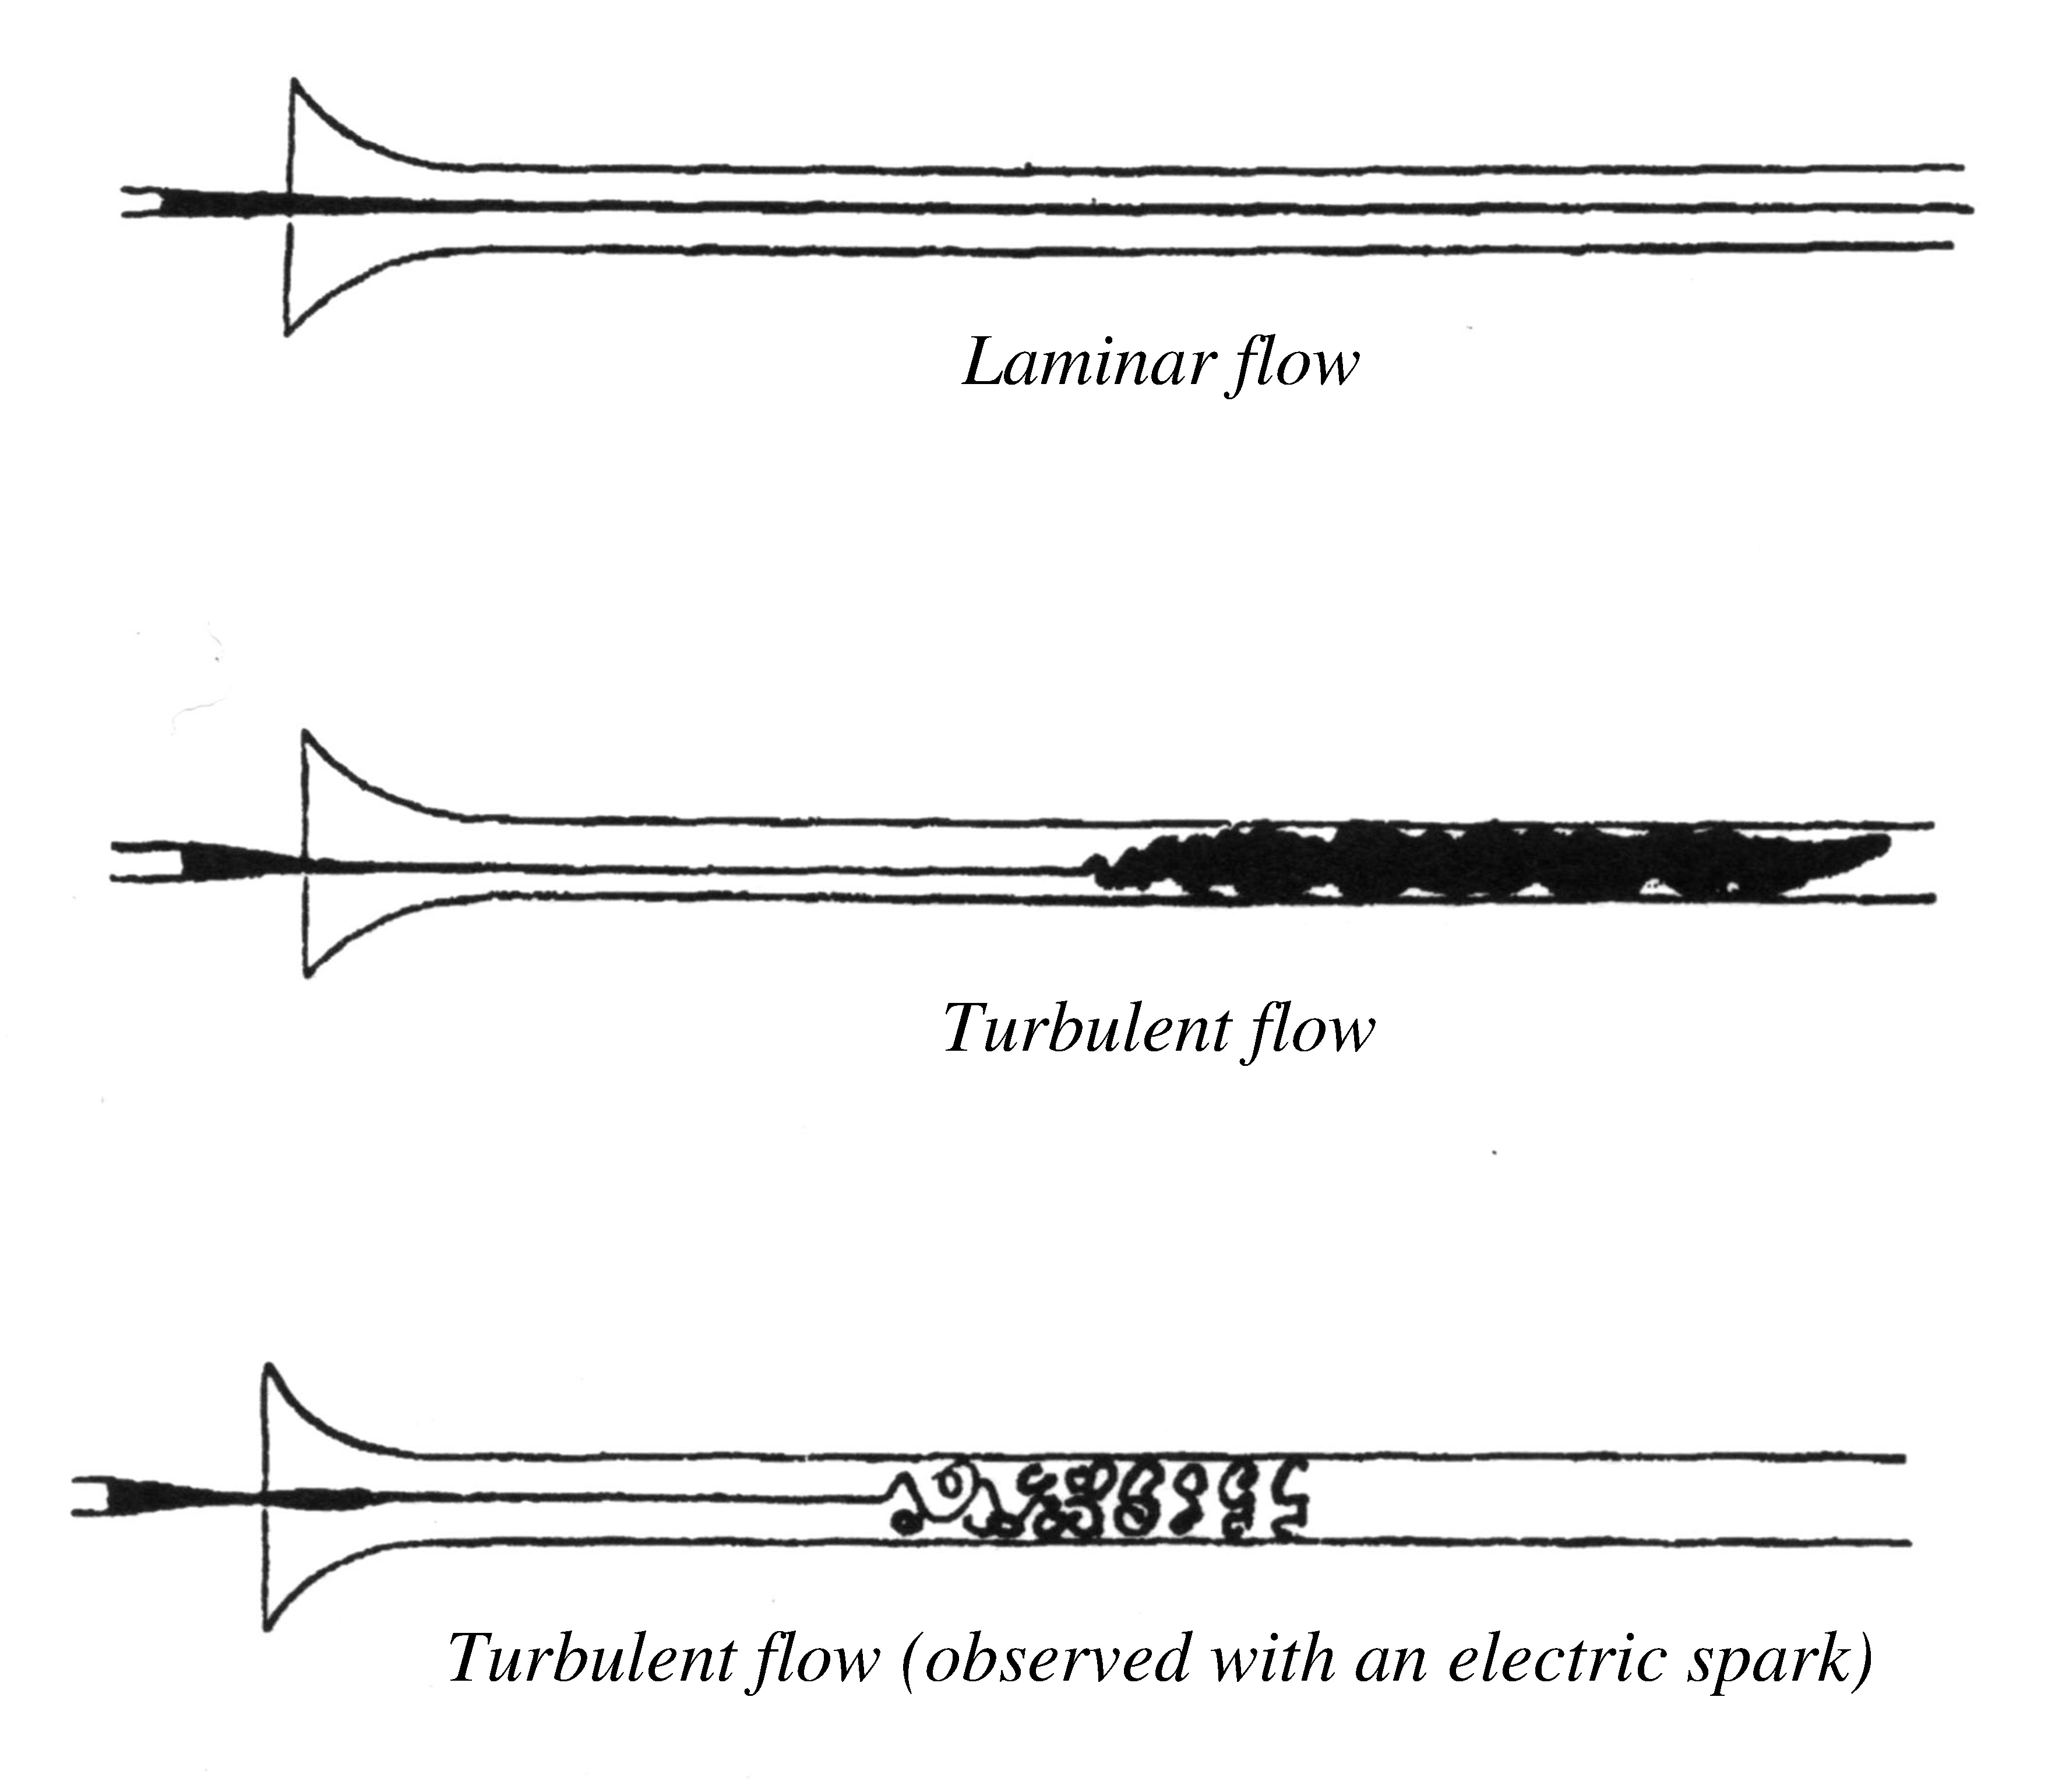
\includegraphics[width=0.5\textwidth]{clase06/Re_observacion.pdf}
\caption{Resultados de Reynolds. Arriba: flujo laminar. Al medio: flujo turbulento. Abajo: flujo turbulentoobservado con una chispa eléctrica.}
\label{fig:Re_observacion}
\end{figure}

Reynolds concluyó que el flujo cambia de laminar a turbulento a $Re$ entre 2000 y 13000, dependiendo del cuidado que se tiene en la disrupción del flujo (ya sea por tener entradas muy abruptas, como vibraciones).
Esto es algo que podíamos imaginar a partir del análisis que hicimos de la ecuación de Navier-Stokes adimensionalizada.

Para estudiar las estructuras que aparecen en la transición a la turbulencia vamos a utilizar el flujo sobre una placa como nuestro problema modelo.
Cabe destacar que el flujo sobre una placa plana genera lo que se conoce como una capa límite. 
Capa límite es un tema que no hemos pasado en este curso aún, pero solamente es necesario saber que el fluido tendrá velocidad 0 sobre la placa, y irá paulatinamente creciendo a medida que nos alejamos de ella hasta llegar a la velocidad con que viene el flujo al infinito $U_\infty$, como lo muerstra la Figura \ref{fig:capa_limite}.
%
\begin{figure}[h!]
\centering
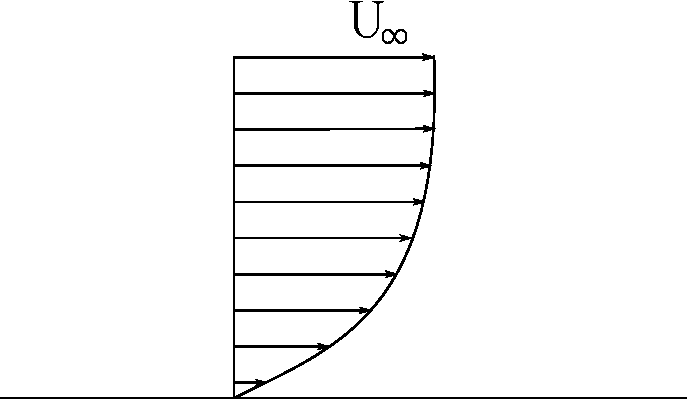
\includegraphics[width=0.5\textwidth]{clase06/capa_limite.pdf}
\caption{Velocidad sobre una placa plana.}
\label{fig:capa_limite}
\end{figure}

Visto desde arriba, la capa límite hace una transición a turbulencia de la forma que muestra la Figura \ref{fig:transicion_turbulencia}.
A continuación haremos una pequeña descripción de cada una de estas etapas.
%
\begin{figure}[h!]
\centering
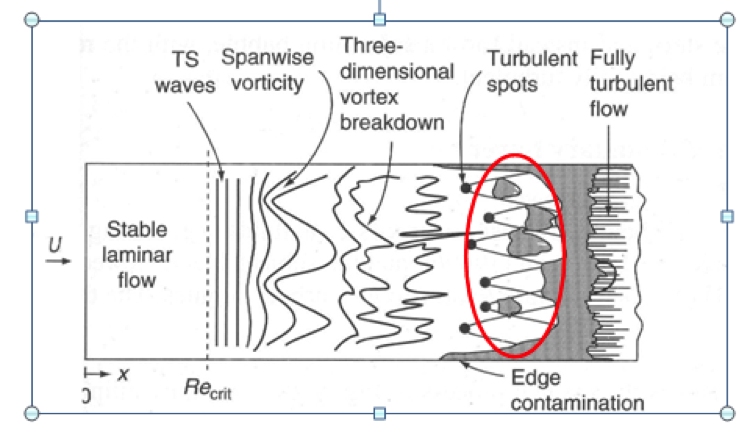
\includegraphics[width=0.5\textwidth]{clase06/transicion_turbulencia.png}
\caption{Transición a turbulencia sobre una placa plana. \emph{Fuente: F. White, Viscous Fluid Flow (2006)}}
\label{fig:transicion_turbulencia}
\end{figure}

\paragraph*{Ondas de Tollmien-Schlichting}
Es la primera indicación de inestabilidad del flujo laminar. 
Estas ondas tienen una naturaleza bidimiensional, ya que son relativamente constantes a lo largo del eje que cruza a lo ancho de la placa.
Inicialmente son prácticamente imperceptibles, pero van creciendo aguas abajo hasta que las nolinealidades de la ecuación de Navier-Stokes comienzan a hacerse notar, generando movimientos en otras direcciones.
Las ondas T-S llegan a ser de \~1-2\% de $U_\infty$.

\paragraph*{Vorticidad a lo ancho de la placa}
Debido a que la no-linealidad toma fuerza, se pierde la bidimiensionalidad del flujo bajo las ondas T-S, y comenzamos a ver variaciones en la vorticidad a lo ancho de la placa.
Inicialmente las variaciones son pequeñas, sin embargo rápidamente toman fuerza y las diferencias en vorticidad a lo largo una misma línea que va hacia adentro puede ser 4 a 5 veces.
Eventualmente, las líneas de vorticidad se tornan irregulares, con vorticidad que se alinea con las líneas de flujo.

\paragraph*{Puntos de turbulencia}
Es la última etapa antes de la turbulencia total.
Las líneas de vorticidad, que se encuentran estiradas, comienzan a romperse en unidades más pequeñas de forma prácticamente random. 
La turbulencia aparece en forma de puntos o núcleos en tiempos y ubicaciones random, y se dispersa aguas abajo en un ángulo entre $8^\circ$ y $10^\circ$.

\section*{La ecuación promediada de Reynolds}

Un flujo turbulento es inherentemente desordenado, sin embargo, 

 
\end{document}
